\documentclass[tikz,border=2pt]{standalone}
\usetikzlibrary{arrows.meta,positioning}

\begin{document}
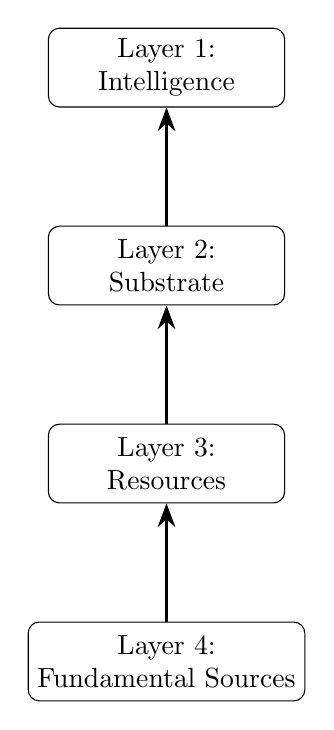
\begin{tikzpicture}[node distance=1.5cm, every node/.style={draw, rectangle, rounded corners, align=center, minimum width=3cm, minimum height=1cm}]
    \node (layer1) {Layer 1:\\ Intelligence};
    \node (layer2) [below=of layer1] {Layer 2:\\ Substrate};
    \node (layer3) [below=of layer2] {Layer 3:\\ Resources};
    \node (layer4) [below=of layer3] {Layer 4:\\ Fundamental Sources};
    \draw[-{Stealth[length=3mm]}, thick] (layer4.north) -- (layer3.south);
    \draw[-{Stealth[length=3mm]}, thick] (layer3.north) -- (layer2.south);
    \draw[-{Stealth[length=3mm]}, thick] (layer2.north) -- (layer1.south);
\end{tikzpicture}
\end{document}
